% 目次の挿入
\tableofcontents
\newpage

% ヘッダーカスタマイズ
\pagestyle{fancy}
\fancyhf{}
\fancyhead[L]{DLITE3:Technology that supports people's lives without boundaries}
\renewcommand{\headrulewidth}{0pt}
\makeatletter
\let\ps@plain\ps@fancy
\makeatother
% ヘッダーの下に空白を追加
\setlength{\headsep}{20pt}

\chapter{はじめに}
\section{背景}
適当な例で本文を書いていくので、chapterやsectionを含め本文を自由に改変してください。\\
\noindent\space
私たちは、普段日常生活で木々の揺らぐ音や、空の色など様々な自然に触れる機会があり、無意識のうちに自然を楽しんでいる。しかし、視覚や聴覚に障害を持つ人は自然の音を聞くことや景色を見ることが難しい。そのため、自然を最大限楽しむことができないと考えた。
\begin{figure}[h!]
  \centering
  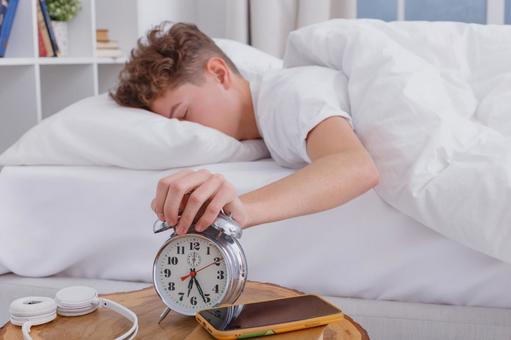
\includegraphics[width=0.8\textwidth]{pages/report/images/alarm-stopping.jpeg}
  \caption{目覚ましの停止が困難な図}
  \label{fig:sample}
\end{figure}
\writer{伊丸岡朝陽}

\section{先行研究}
近年、障害者支援として、エンターテインメントの観点から支援する取り組みが広まりつつある。ピクシーインダストリーズ(2018)\cite{SOUNDHUG}は、「SOUND HUG」(サウンドハグ)というデバイスを開発している。
このデバイスは⾳楽をマイクで拾い、リアルタイムに光や振動を変換させることにより、聴覚障害の方が視覚や触覚情報を受け取りながら、音楽鑑賞会を楽しむことができる。
この事例をもとに、自然を別の形式に変換させることで、視覚障害や聴覚障害を抱える方も自然を最大限楽しむことができるのではないかと考えた。
\writer{伊丸岡朝陽}

\section{研究動機}
\noindent\space
私たちのグループでは、まず障害を抱えている人がどのような問題を抱えているのかを一部体感するために、フィールドワークから行った。
フィールドワークの内容は以下2つを室内、屋外で行った。
% フィールドワークの内容
\begin{enumerate}
  \item イヤフォンで耳を塞いだ状態で外部の音を完全に遮断し徘徊する。
  \begin{itemize}\item[-] 聴覚情報の遮断\end{itemize}
  \item 手で目を覆った状態で視覚情報を遮断し徘徊する。5分間目を瞑った状態で座る。
  \begin{itemize}\item[-] 視覚情報の遮断\end{itemize}
\end{enumerate}
その結果、以下のことに気付いた。
% フィールドワークの結果
\begin{itemize}
  % ===== 聴覚 =====
  \item 聴覚情報の遮断
  \begin{itemize}
    \item 室内
    \begin{itemize}
      \item 一緒に歩いている人の足音が聞こえないため、視界から外れたときに足音が聞こえなくてついてきているのか分からない。
      \item 曲がり角や階段の頂上付近で人が来ているのか足音から分からず、普段より警戒した。
      \item 自分のコツコツとした足音が聞こえず、歩いている感がない。
    \end{itemize}
    \item 屋外
    \begin{itemize}
      \item 風の音や風が吹くことによる音(葉っぱが揺らぐ音など)が聞こえず、涼しさや季節感を感じられにくかった。
      \item 芝生を歩いたが、コンクリートよりも歩いたときの感触が強いので、歩いているという感覚が強い。
      \item 道路を渡る時に車が来ているのか音での判別ができず若干危険。
    \end{itemize}
  \end{itemize}
  \newpage
  % ===== 視覚 =====
  \item 視覚情報の遮断
  \begin{itemize}
    \item 室内
    \begin{itemize}
      \item 会話をする中で説明をする際にジェスチャーが使えなくて不便。
      \item 音に集中するため音の聞こえ方がより立体的になる。
      \item 会話のとき、ジェスチャーが使えないので簡単な「上」や「下」を使って説明することがあった。
    \end{itemize}
    \item 屋外
    \begin{itemize}
      \item 花の色が見れない。
      \item 木々の揺れ方は音からある程度は伝わるがどの程度揺れいているのかのイメージがつかみにくい。
      \item 日が昇っているのか沈んでいるのか分からない。
    \end{itemize}
  \end{itemize}
\end{itemize}
これらの結果から、室内では視覚や聴覚の情報が遮断されることで、様々な危険が増えることが分かった。
また屋外では、危険が増えるだけでなく、日常的に触れている自然が感じられにくくなった。
これらを踏まえ、今回は屋外での問題に着目し、障がいの有無に関わらず、自然を楽しむことが出来るようにしたいと考えた。
\writer{伊丸岡朝陽}

\section{目的及び重要性}
布団から一歩も出ずに用意に目覚まし時計を止めることが出来るような方法を考案することで、快適な二度を実現する。
また、快適な二度寝により幸福度が増し、生活の質が向上することが期待されるとともに、人生を豊かにすることが出来ると考える。
\writer{未来太郎}

\chapter{関連研究}
\section{必要なスキル}
遠隔操作により、ワイヤレスで目覚まし時計を操作することが出来るような方法を考案することが必要である。
また、そのためには以下の技術の習得が必要であると考える。
\begin{itemize}
    \item ワイヤレス通信技術
    \item マイコン制御技術
    \item 電子回路設計技術
    \item スマホアプリ開発技術
\end{itemize}
\writer{未来太郎}

\section{解決方法・手法}
視覚や聴覚に障害のある方が自然を体感できるための手法として、2つ挙げられる。
1つ目として視覚の障害を持つ方には、自然の景色をその景色から連想できる音楽に変換する。
2つ目は、聴覚の障害をもつ方には 自然の音を集音し、その音から連想できるビジュアルアートを生成する。
これら2つのの手法はどちらも障害の有無にかかわらず、自然の新たな楽しみ方としての価値を創造できる。
\writer{伊丸岡朝陽}

\chapter{本プロジェクト学習の目標}
\section{最終的な目標}
本プロジェクト学習では、目覚まし時計をスマホで操作し遠隔で停止させるアプリ、デバイスを開発することで、快適な二度寝を実現することを目標とする。
またそれにより、生活の質が向上し、幸福度を増加させることを最終的な目標とする。
\writer{未来太郎}

\chapter{目的を達成するための手法・手段}
\section{考案したアイデア}
考案したアイデアについて述べる。
\writer{未来太郎}

\section{新しい解決方法・手法}
解決方法の新規性について述べたりする。
\writer{未来太郎}

\section{用いる技術}
上記を実現するために用いる技術について述べる。
\writer{未来太郎}

\chapter{結果}
\section{手法な結果}
どんな結果が得られたのかを事実に基づいて述べる。
\writer{未来太郎}

\chapter{考察}
\section{得られた成果}
本プロジェクト学習を通じてどのような成果を得られ、どのような効果が発生したのかについて考察する。
\writer{未来太郎}

\section{妥当性}
得られた結果は妥当かどうかについて述べる。
\writer{未来太郎}

\section{課題点}
用いた手法、技術では得られなかったことについて述べる。
\writer{未来太郎}

\section{本学との関連性}
本学のカリキュラムや講義科目との関係や関連性について述べる。
\writer{未来太郎}

\section{拡張性}
本プロジェクト学習を拡張することでどのような新たなテーマが考えられるかについて述べる。
\writer{未来太郎}

\section{今後の展望}今後の展望として、以下を実現したいと思う。
\subsection{}使用者の好みに合わせることができるデバイスのカスタマイズ性を実現したい。
\subsection{}視覚や聴覚に障害を持つ方に実際に使ってもらい、フィードバックをもらいたい。
\subsection{}自然に新たな価値を見出すことで、障害の有無にかかわらず、自然を楽しめるよう実現したい。
\writer{伊丸岡朝陽}

\newpage\clearpage
\vspace*{-20pt}
\addcontentsline{toc}{chapter}{参考文献}  % 目次に「参考文献」を追加
\printbibliography[segment=\therefsegment,heading=subbibliography]
